\setcounter{chapter}{5}
\chapter{Test d'ipotesi}

\section{Test del $\chi^2$}

Consideriamo un campione di N misure $\{(x_i,y_i)\}_i^N$ IID legate tra loro da una funzione $y =\psi(x,\vec{\theta})$ avremo che le misure campionate rispetto alla variabile aleatoria y, possono essere riscritte come $y_i = \psi(x,\vec{\theta}) + \epsilon_i$ dove $\epsilon$ ipotizziamo essere una variabile aleatoria la cui $pdf(\epsilon)$ segue una distribuzione di probabilit\`{a} Gaussiana. Nell'ipotesi in cui valga il TCL per le $\epsilon_i$, si ha che il $Q^2$ associato alle misure e il modello segue la distribuzione di $\chi^2(N-k)$.

 
\begin{figure}[ht]
\vspace{0.2in}
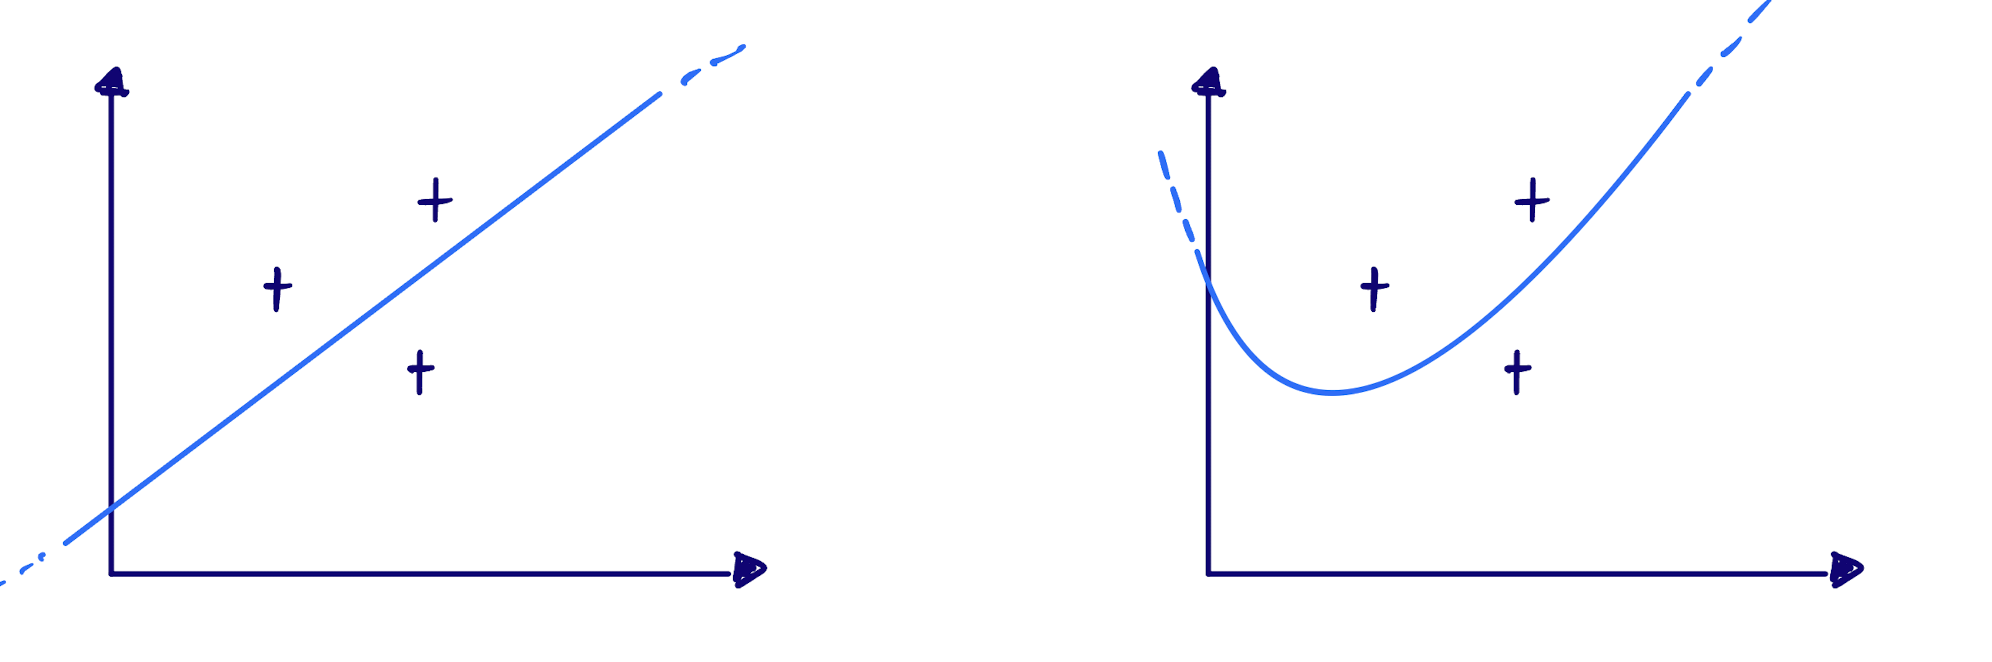
\includegraphics[scale = 0.35]{compa}	
\centering
\vspace{0.1in}
\caption{Due modelli differenti che interpolano lo stesso campione di dati.}
\end{figure} 
\noindent Nel caso di destra in figura 6.1 gli scarti quadratici sono minori, mentre in quello di destra sono pi\`{u} grandi, di conseguenza possiamo aspettarci che il valore di aspettazione della distribuzione di $\chi^2$ del modello di sinistra sia pi\`{u} grande di quello di destra. Definiamo il modello non corretto (quello di sinistra) $H_1$ e il modello corretto (quello di destra) $H_0$, la domanda che possiamo porci \`{e}: " Se partiamo da due ipotesi $H_1$ e $H_0$ e non sappiamo quale delle due sia corretta, come facciamo a determinare quella che descrive meglio la realt\`{a} sperimentale? ". \newline
Introduciamo una nuova quantit\`{a} definita \textbf{p-value} che ha la seguente espressione :
\vspace{0.2in}

\begin{minipage}{.4\textwidth}
	\begin{equation}
		\text{p-value} = \int_{\overline{Q}^2}^{\infty}\chi^2(N-k)d\chi^2 
	\end{equation}
  \end{minipage}
  \begin{minipage}{.4\textwidth}
    \centering
    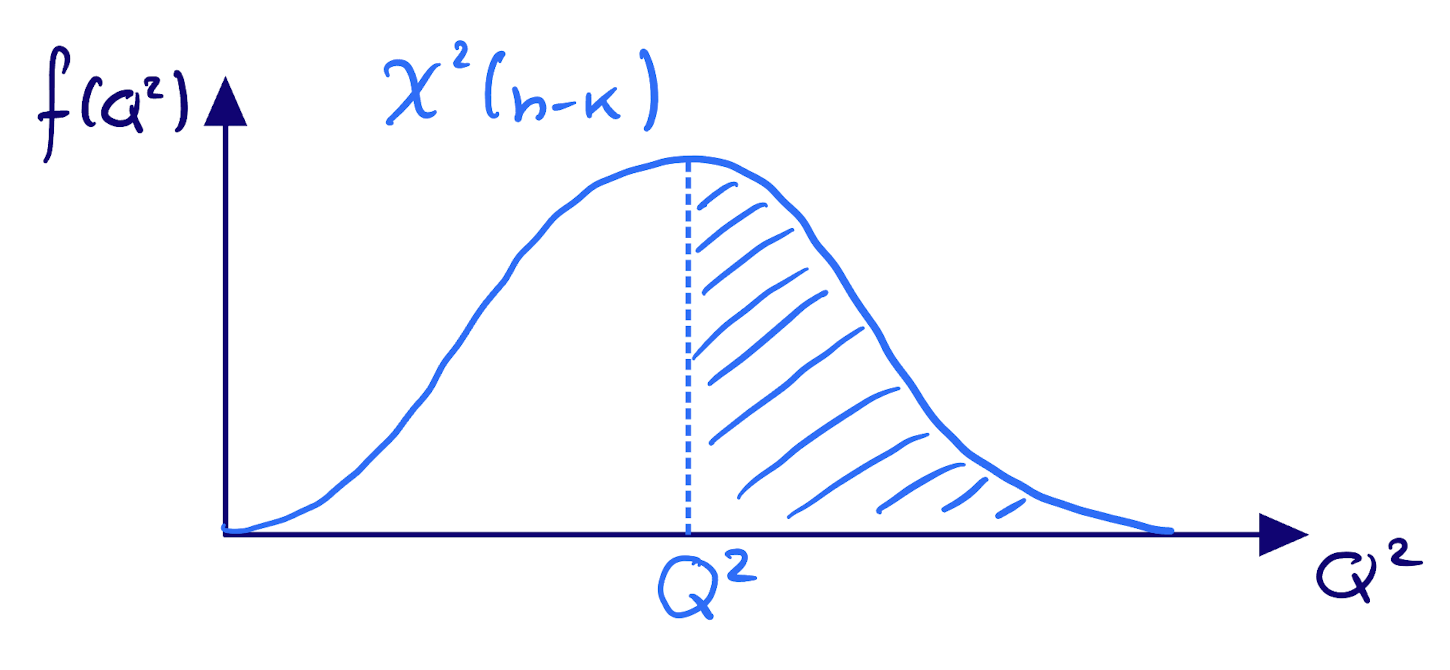
\includegraphics[scale = 0.3]{pvalue}	
  \end{minipage}
\vspace{0.2in}

\noindent la quantit\`{a} cos\`{i} definita risulta essere una misura di probabilit\`{a}. Per rispondere alla domanda precedente fissiamo una soglia di tolleranza del p-value oltre alla quale i valori ottenuti risultano essere dei \textbf{falsi negativi}. Riprendendo i modelli $H_0$ e $H_1$ che definiamo rispettivamente \textbf{null hypothesis} e \textbf{alternative hypothesis} poich\`{e} $H_1$ ha un valore di aspettazione pi\`{u} grande di $H_0$, fissata una soglia del p-value, e definita una statistica x associata al $\chi^2(x \vert N-k)$ avremo che:
\begin{itemize}
	\item H0 \`{e} rigettata se x cade nella regione in azzurro $\omega_\alpha^* $ in figura 6.2
	\item H0 \`{e} accettata se x cade nella regione in verde $\omega_\alpha$ nella figura sottostante.
\end{itemize}
\begin{figure}[ht]
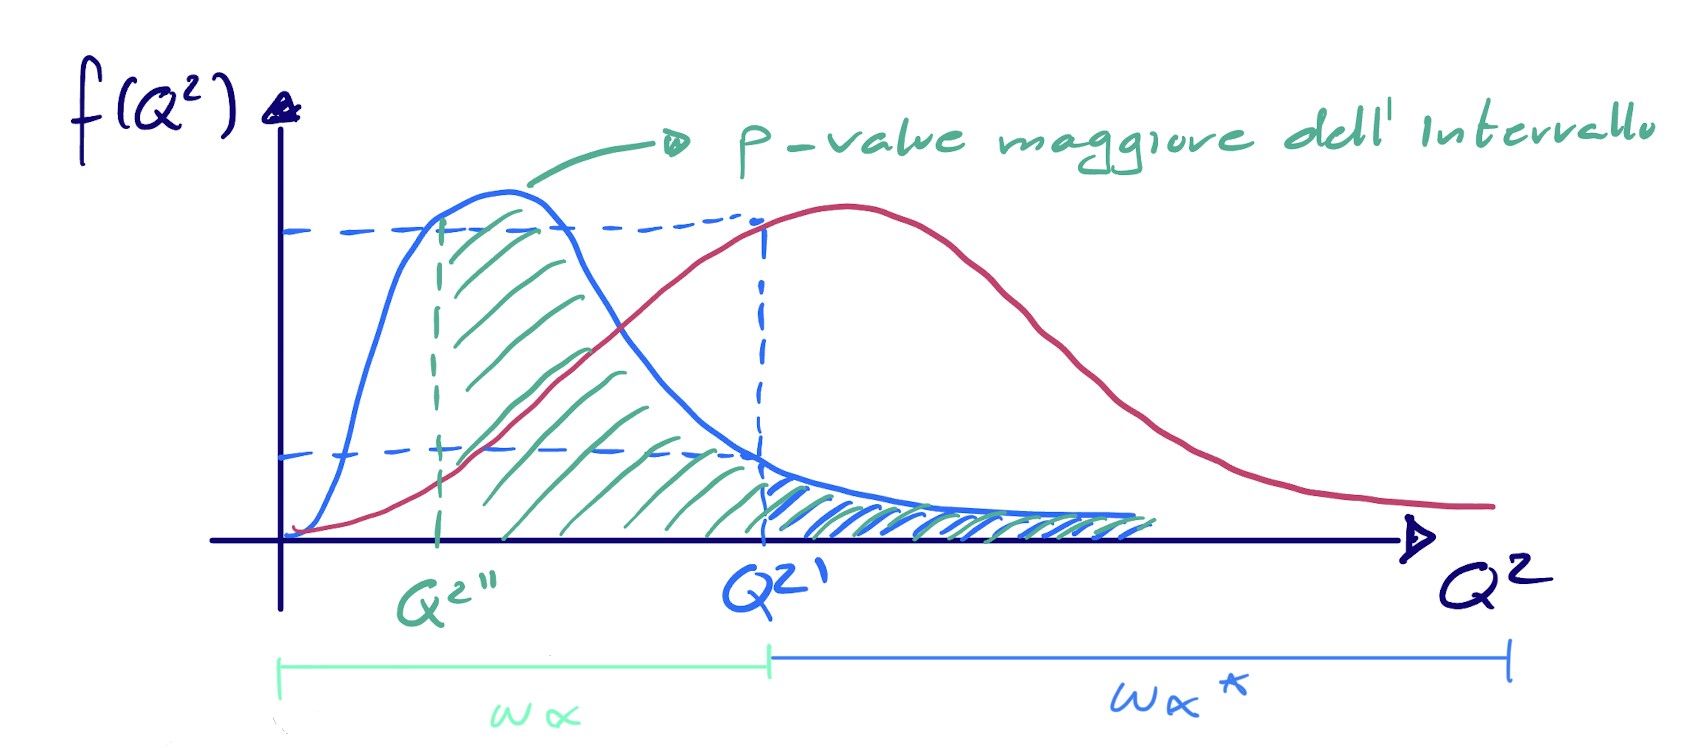
\includegraphics[scale = 0.4]{hypo}	
\centering
\end{figure}
Su quanto discusso fino ad ora possiamo fare le seguenti osservazioni:
\begin{itemize}
	\item I minimi quadrati calcolano il $Q^2$ (e anche la ML calcola i parametri $\hat{\theta}$ da cui si può calcolare il $Q^2$);
	\item Test del $\chi^2$ funziona perché conosciamo la p.d.f. del $Q^2 \Rightarrow \sigma^2$  deve essere nota e ben stimata;
	\item Test del $\chi^2$ è un test integrale $\Rightarrow$ Somma gli scarti su tutti gli eventi.
\end{itemize}

\subsubsection{Esempio}

\begin{wrapfigure}{l}{0.\textwidth}
\centering
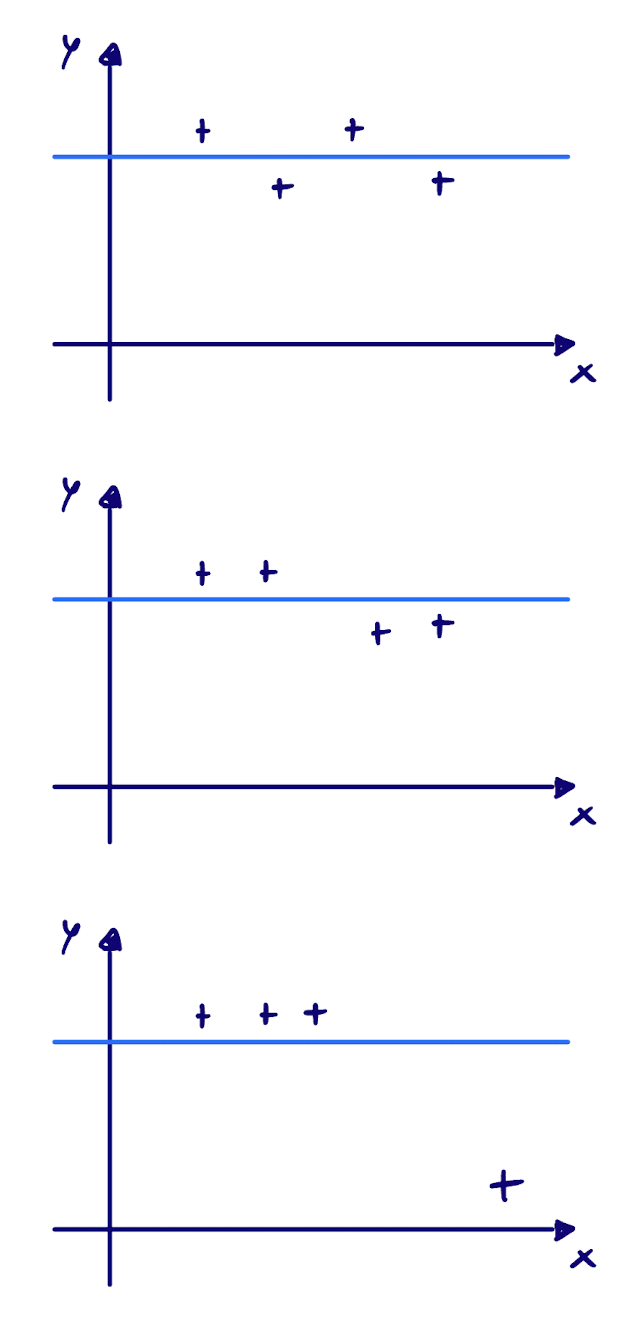
\includegraphics[scale = 0.5]{esempio}	
\end{wrapfigure}

Assumiamo che il p-value sia accettabile ovvero maggiore
dell'intervallo di confidenza. Consideriamo gli stessi punti 
riorganizzati in un modo diverso, ma con stesso scarto quadratico.
I due set di dati con y differenti hanno lo stesso p-value.

Essendo che il test del $\chi^2$ ha una forma integrale, se
graficamente si osserva una distribuzione differente delle
misure, il test non lo tiene in considerazione.

Se consideriamo una dispersione delle misure come nella terza figura e
assumiamo che abbia il medesimo p-value delle altre due, si ha
che il test non considera che i dati diminuiscono di valore lungo l'asse delle ordinate e dunque si ottiene un \textbf{falso positivo}, ovvero p-value \`{e} verificato, ma il modello non descrive adeguatamente il comportamento dei dati sperimentali.

Il fatto che il test del $\chi^2$ abbia forma integrale limita la generalit\`{a} con cui possiamo decidere se il risultato ottenuto sia affidabile o meno.

\begin{wrapfigure}{r}{0.\textwidth}
\centering
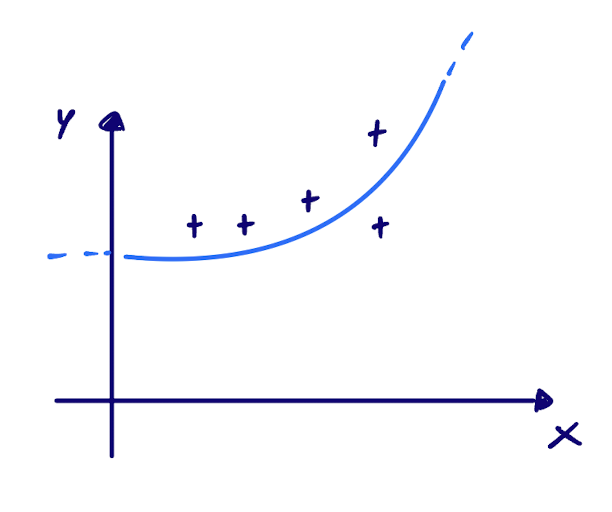
\includegraphics[scale = 0.5]{overfit}	
\end{wrapfigure}

\noindent Ipotizziamo di avere un fit che ha $Q^2$ = 0 e p-value-1,
ovvero i dati vengono interpolati perfettamente , questo non è
un buon risultato. Si ha un caso di overfitting, dove si sono introdotti così tanti parametri che
il risultato del fit si \`{e} completamente adattato alle misure, perdendo qualsiasi
capacit\`{a} di generalizzare il modello. 

\subsection{Applicazione del test di $\chi^2$}

Se il modello \`{e} corretto $y = \psi(x,\vec{\theta})$, allora il metodo dei MQ fornisce una stima dei parametri $\vec{\theta}$ che lo descrivono. Il valore stimato dei parametri rappresenta il punto di minimo del funzione di $Q^2_{min} = Q^2(x,\vec{\theta}_{MQ})$ rispetto al campione sperimentale, tale punto di minimo coincide anche con il massimo della distribuzione di $\chi^2$ se pdf($\epsilon$) seguono una distribuzione gaussiana, che \`{e} dato da $E[Q^2] = N-k$ e quindi $Q^2_{min} = N-k$. \newline
Il $\chi^2$ ridotto \`{e} definito come $\chi^2_{0} = \frac{\chi^2}{ndof}$ ci\`{o} implica che per $\chi^2_{min} = Q^2_{min}$ il ridotto \`{e} $\chi^2_0 \sim 1$. \newline
Se il valore del $\chi^2_{min}$ \`{e} lontano dal suo valore di aspettazione N-k, possiamo concludere che alcune delle ipotesi precedenti non sia corrette e dunque \textbf{i dati non confermano il modello}.

\section{Errori di test statistici}

\subsection{Errori del $I^{\circ}$ tipo}

Un errore del primo tipo rappresenta il numero di casi veri per la null hypothesis Ho che scartiamo fissata una soglia del p-value.

\vspace{0.3in}
\begin{minipage}{.4\textwidth}
	\begin{equation}
		\alpha = \int_{\overline{Q}^2}^{\infty}\chi^2(N-k)d\chi^2 
	\end{equation}
  \end{minipage}
  \begin{minipage}{.4\textwidth}
    \centering
    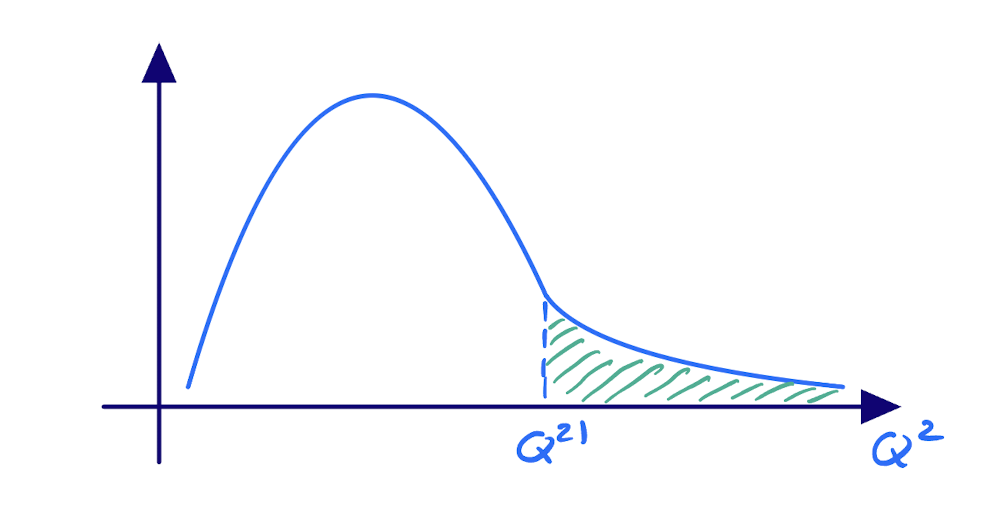
\includegraphics[scale = 0.4]{size}	
  \end{minipage}
\vspace{0.2in}

Il termine $\alpha $ prende il nome di \textbf{size del test}. 

\subsection{Errori del $II^{\circ}$ tipo}

 Un errore del secondo tipo rappresenta la probabilit\`{a} di accettare H0 quando \`{e} vera H1, in questo caso si parla di \textbf{falsi positivi}. 
 \vspace{0.2in}
 
\begin{minipage}{.4\textwidth}
	\begin{equation}
		\beta = \int_{Q^2}^{\overline{Q}^2}\chi^2(N-k)d\chi^2 
	\end{equation}
  \end{minipage}
  \begin{minipage}{.4\textwidth}
    \centering
    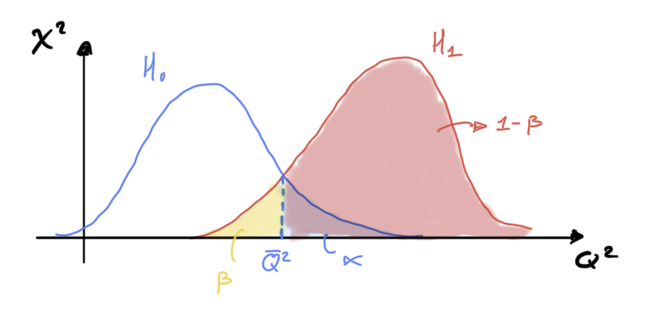
\includegraphics[scale = 0.3]{powertest}	
  \end{minipage}
\vspace{0.2in}

Si sta commettendo un errore poich\`{e} se H1 \`{e} la forma funzionale sbagliata il fit dei dati supera ugualmente il test del $\chi^2$. 

\noindent Il termine $1-\beta$ prendere il nome di \textbf{power del test} e restituisce la probabilit\`{a} di rifiutare $H_0$ quando $H_1$ \`{e} vera.
\newline

\noindent Fissate le due ipotesi alternative e definiti gli intervalli di confidenza, se si assume che l'errore di tipo uno sia quello pi\`{u} grave si procede scegliendo la percentuale di falsi negativi che si reputa accettabile e si cerca di definire gli intervalli $\omega_\alpha$ e $\omega_\alpha^*$ in modo tale che $\beta$ sia il minore possibile (minor caso di falsi positivi). Il test cos\`{i} descritto viene definito il pi\`{u} potente per un determinato valore di soglia del p-value.

\section{Test di Kolgomorov-Smirnov}

Consideriamo un insieme di N misure della stessa grandezza fisica X vogliamo testare l'ipotesi $H_0$ che siano campionamenti di una determinata pdf-modello. Una possibilit\`{a} \`{e} di usare il test del $\chi^2$ applicandolo agli istogrammi costruiti con le misure raccolte e la pdf-modello. Tale procedura \`{e} corretta, ma richiedere di binnare i dati e dunque si ha una perdita d'informazione, inoltre l'esito del test pu\`{o} dipendere dal binning scelto per la costruzione degli istogrammi.

L'alternativa \`{e} data dal test di \textbf{Kolgomorv-Smirnof} che confronta le due distribuzioni cumulative (dati - pdf-modello) e in questo modo sfrutta tuta l'informazione contenuta nei dati.


\subsection{Ricostruzione della cumulativa}

Consideriamo N misure ordinate in senso crescente, ricostruiamo la distribuzione cumulativa della pdf-modello, definendo una funzione a gradini $S_n$ rispetto ai dati del campione poich\`{e} sono presenti dei buchi nell'informazione.
\vspace{0.2in}

\begin{minipage}{.4\textwidth}
	\begin{align*}
S_n(x) = 
	\begin{cases}
	n \quad x_i < x < x_{i+1} \\
	0 \quad \quad \quad \text{altrimenti}\\
	\end{cases}
\end{align*}
  \end{minipage}
  \begin{minipage}{.4\textwidth}
    \centering
    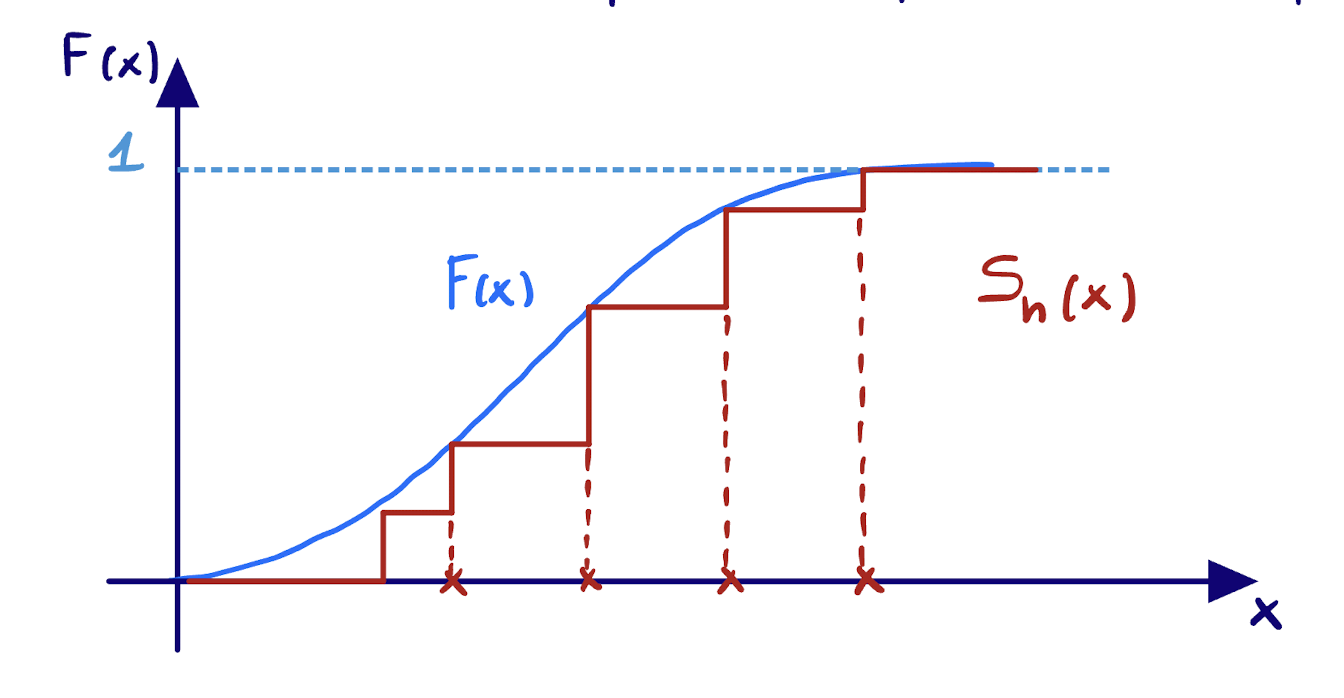
\includegraphics[scale = 0.3]{step}	
  \end{minipage}
\vspace{0.2in}

Ci si domanda quanto bene $S_n$ approssimi la cumulativa F(x), la risposta \`{e} che dipende dal numero di misure contate prima del gradino successivo e quindi da come si scelgono gli intervalli. Di primo impatto si potrebbe pensare di misurare la distanza tra i gradini e la cdf continua per dare una stima dell'approssimazione, il problema \`{e} che se sono presenti scarti significativi tra le due grandezze questo si rifletterebbe sulla stima complessiva in modo negativo. Per effettuare la misura consideriamo il discriminante:
\begin{equation*}
	D_n = \sup_{x} \vert S_n(x) -F(x) \vert 
\end{equation*}
 e si dimostra che la distanza $d_n = \sqrt{n}D_n$ per $n \rightarrow \infty$ converge alla distribuzione F(x).
 Il test consiste nel confrontare lo scarto massimo:
 \begin{equation*}
 	\delta = Max \{D_n(x)\}
 \end{equation*}
 con una grandezza di riferimento $\delta_0$. Se $\delta > \delta_0$ l'ipotesi di compatibilit\`{a} viene rigettata. Il valore di $\delta_0$ \`{e} scelto in base alla probabilit\`{a} che la variabile casuale $\delta$ sia maggiore di $\delta_0$ quando il modello \`{e} corretto.
 \begin{equation*}
 	P(\delta > \delta_0 \vert H_0) = \alpha
 \end{equation*}
 Il test \`{e} utile per confrontare due campioni di dati al fine di determinare se provengono dalla stessa popolazione.
 
 \section{Confronto di una misura con il valore di riferimento}
 \subsection{Distribuzione di t-student}
 Si consideri un campione di N misure di cui si \`{e} calcolata la media campionaria $\overline{x} = \frac{1}{N} \sum x_i$ e si supponga di conoscere $\sigma_i$ delle singole misure e $E[x] = \mu$, allora la media aritmetica $\overline{x}$ \`{e} per il TCL \`{e} distribuita come una gaussian G($\overline{x}$,$\mu$, $\frac{\sigma}{\sqrt{N}}$). Come facciamo a dire che $\overline{x}$ e ${\mu}$ sono sufficientemente vicine tra loro rispetto alle incertezze ?
 \newline
 Per determinare la distanza tra le grandezze definiamo la distribuzione t-student data dalla variabile aleatoria:
 
 \begin{equation*}
 	t = \dfrac{\vert \overline{x} - \mu\vert }{\frac{\sigma}{\sqrt{N}}}
 \end{equation*}
 definita rispetto al caso descritto nelle righe precedenti. In generale la t-student per un parametro \`{e} data da:
 \begin{equation}
 	t = \dfrac{\vert \hat{\theta}^* - \theta_t \vert}{\sigma_{\theta^*}}
 \end{equation}
 
 Notare che nel caso in cui si conoscano a priori l'incertezza della misura che si sta confrontando, dunque non si \`{e} ottenuta mediante un processo statistico si ha che la pdf(t) \'{e} Gaussiana.
 Se $\overline{x}$ segue una pdf Gaussiana e $Q^2 \sim \chi^2(N-1)$ la distibuzione di t-student ha la seguente forma funzionale.
 
 \begin{equation}
 	f(t,\nu = N-1) = \dfrac{1}{\sqrt{n\nu}} \cdot \dfrac{\Gamma({\frac{\nu+1}{2}})}{\Gamma(\frac{\nu}{2})} \cdot \Big (1 + \frac{t^2}{\nu} \Big) ^{-(\frac{\nu+1}{2})}
 \end{equation}
 
 \subsubsection{Propriet\`{a} della distribuzione}
 \begin{align*}
 	\begin{matrix}
 		\mu = E[t] = 0 & \quad \quad & \gamma_1 = 0 \\
 		\\
 		\sigma^2 = V[t] = \frac{\nu}{\nu-2} \quad \nu > 2 & \quad \quad & \gamma_2 = \frac{6}{\nu-4} \quad \nu > 4
 	\end{matrix}	
 \end{align*}
 \newline
 Per $\nu \rightarrow \infty$ la distribuzione diventa Gaussiana. Si osserva che la pdf della t-student \`{e} un po' pi\`{u} larga della distribuzione Gaussiana (fig 6.2).
 
  
\begin{figure}[ht]
\vspace{0.1in}
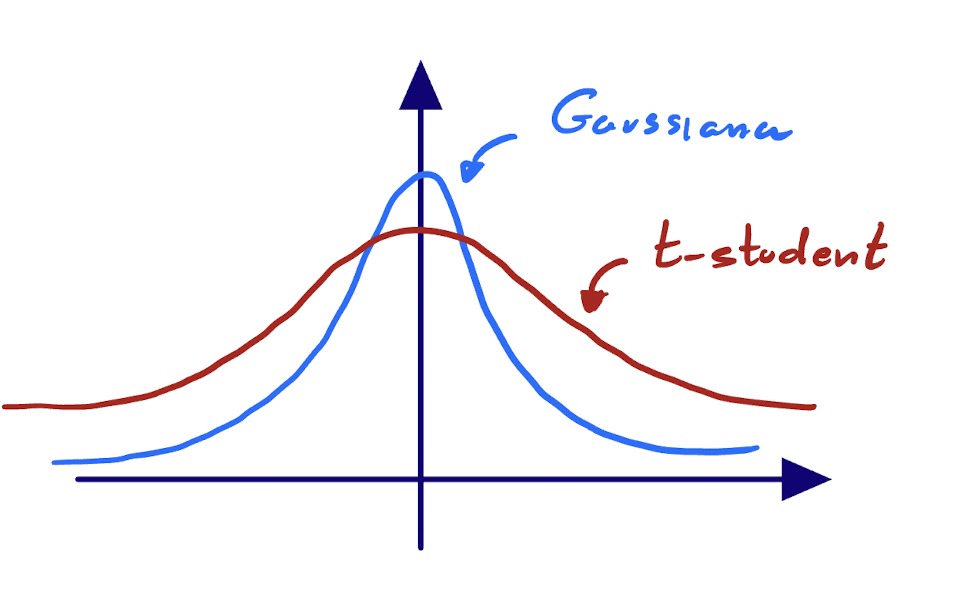
\includegraphics[scale = 0.4]{student}	
\centering
\vspace{0.1in}
\caption{Confronto distribuzioe di Gauss e t-student}
\end{figure}
In generale possiamo vedere la distribuzione della t-student come il rapporto tra una Gaussiana normalizzata e la radice di  $\frac{\chi^2}{N-1}$.
\begin{equation*}
	t = \dfrac{\vert \overline{x} - \mu \vert}{\Big [{\dfrac{\hat{\sigma}^2}{N}} \Big ]^{\frac{1}{2}}} = \textcolor{cyan}{\dfrac{\vert \overline{x} - \mu \vert}{\Big [{\dfrac{\sigma^2}{N}} \Big ]^{\frac{1}{2}}}} \cdot \textcolor{red}{\dfrac{\Big [ \dfrac{\sigma^2}{N} \Big]^{\frac{1}{2}}}{\Big [ \dfrac{\hat{\sigma}^2}{N} \Big]^{\frac{1}{2}}}} = \textcolor{cyan}{\dfrac{\vert \overline{x} - \mu \vert}{\Big [{\dfrac{\sigma^2}{N}} \Big ]^{\frac{1}{2}}}} \cdot \textcolor{red}{\Big [ \dfrac{\chi^2}{N-1} \Big ]^{\frac{1}{2}}}  
\end{equation*}
la parte in azzurro segue la pdf di una Gaussiana normalizzata N(0,1), mentre la parte in rosso segue $\frac{\chi^2}{N-1}$. Dove:
\begin{equation*}
	\textcolor{red}{\dfrac{1}{\Big [ \dfrac{\sigma^2}{\hat{\sigma}^2} \Big ]^{\frac{1}{2}}} = \dfrac{1}{\Big[  \frac{N-1}{\chi^2} \Big ]^{\frac{1}{2}} } = \Big [ \dfrac{\chi^2}{N-1} \Big ]^{\frac{1}{2}}  } 
\end{equation*}
Per la t-student fissato un valore di soglia $t_0$, ci permette di determinare la compatibilit\`{a} tra il valore stimato e quello atteso, se $t>t_0$ allora le due misure risultano essere non compatibili tra loro. Dove gli intervalli di compatibilit\`{a} risultano essere in multipli di deviazioni standard.
\begin{figure}[ht]
\vspace{0.1in}
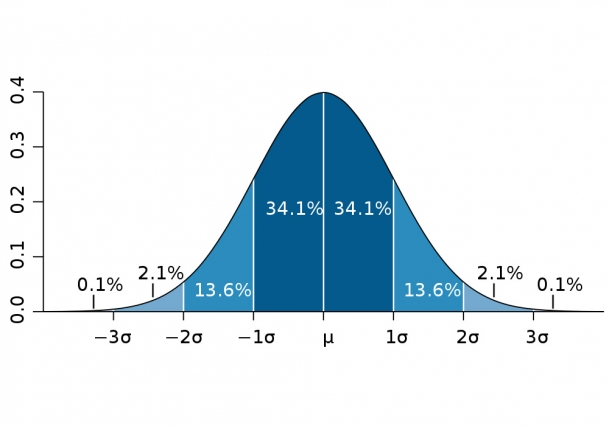
\includegraphics[scale = 0.5]{Bellcurve}	
\centering
\end{figure}

\subsubsection{Confronto tra la stima di due parametri}

La distribuzione di t-student pu\`{o} essere utilizzata non solo per confrontare una misura con un valore atteso, ma anche due stime del medesimo parametro tra loro.

\begin{equation}
	z = \dfrac{\vert \theta^*_1 - \theta^*_2 \vert }{ \Big [\dfrac{\hat{\sigma_1}}{N} +\dfrac{\hat{\sigma_2}}{N} \Big ]^{\frac{1}{2}}}
\end{equation}
dove la pdf(z) \`{e} Gaussiana se $\sigma_1$ e $\sigma_2$ sono senza errore, mentre altrimenti segue una distribuzione di t-student con N-M-2 gradi di libert\`{a}.

\section{Intervalli di confidenza}

Ipotizziamo che lo stimatore $\hat{\theta}$ segue una distribuzione gaussiana G($\hat{\theta},\theta_t,\sigma$) determinato il suo valore $\theta^*$ ci domandiamo quale sia la probabilit\`{a} che tale valore disti $\sigma$ dal valore vero $\theta_t$, ovvero $P[\theta^* \in (\theta_t - \sigma, \theta_t + \sigma)]$ = 0,68. Essendo $\theta^*$ una variabile aleatoria dipendente dal campione di stima possiamo riscrivere l'intervallo di confidenza come $ \theta_t \in (\theta^* - \sigma,\theta^* + \sigma)$ e dunque riscrivere la probabilit\`{a} come $P[\theta_t \in (\theta^* - \sigma, \theta^* + \sigma)]$ = 0,68, dunque si ha un 68 \% di probabilit\`{a} d'intercettare $\theta_t$.
\begin{figure}[ht]
\vspace{0.1in}
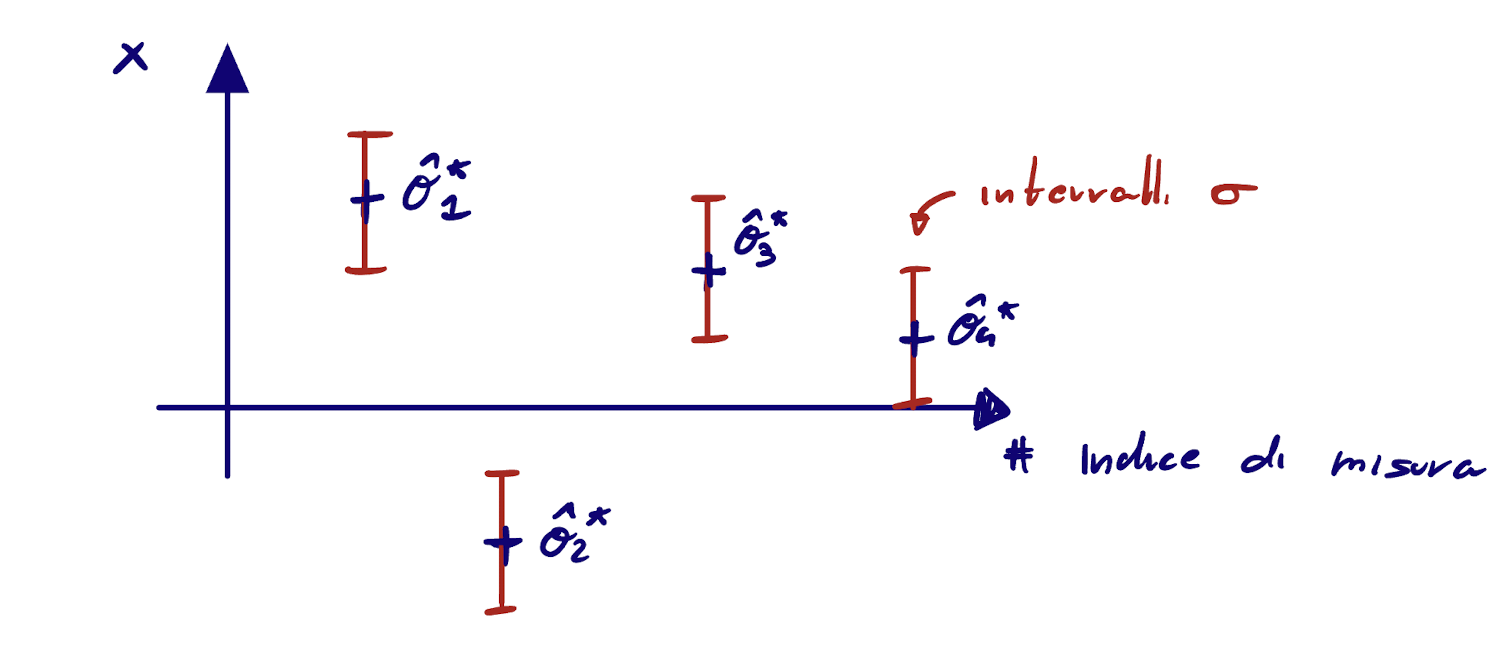
\includegraphics[scale = 0.45]{intervaltheta}	
\centering
\end{figure}

\subsection{Metodo della cintura di confidenza}

Ipotizziamo di non conoscere o non riuscire a determinare la pdf che descrive $\hat{\theta}$, al cambiare di $\theta_t$ cambia anche la pdf di $\hat{\theta}$ e di conseguenza anche gli intervalli di confidenza. Vogliamo determinare un intervallo di confidenza per i parametri stimati $\theta^*$ per farlo applichiamo il seguente metodo:

\begin{itemize}
	\item Per ogni valore di $\theta_t$ definiamo pdf($\hat{\theta} \vert \theta_t$);
	\item Si determinano i punti di pdf($\hat{\theta} \vert \theta_t$) che definiscono un intervallo di confidenza per il $\theta_t$ corrispettico;
	\item Si tracciano due rette parallele che attraversano ciascuna i punti estremanti di ciascun intervallo di confidenza, definendo una banda nel piano $(\theta_t,\theta^*)$ che prende il nome di \textbf{Confidence Band}.
\end{itemize}
Quando si effettua una misura si trova $\theta^*$ e dove tale valore interseca la confidence band, punti
d'intersezione determinano l'intervallo di confidenza di $\theta_t$. Si dimostra che l'intervallo trovato ha copertura uguale a quello scelto per le singole p.d.f.

 
\begin{figure}[ht]
\vspace{0.2in}
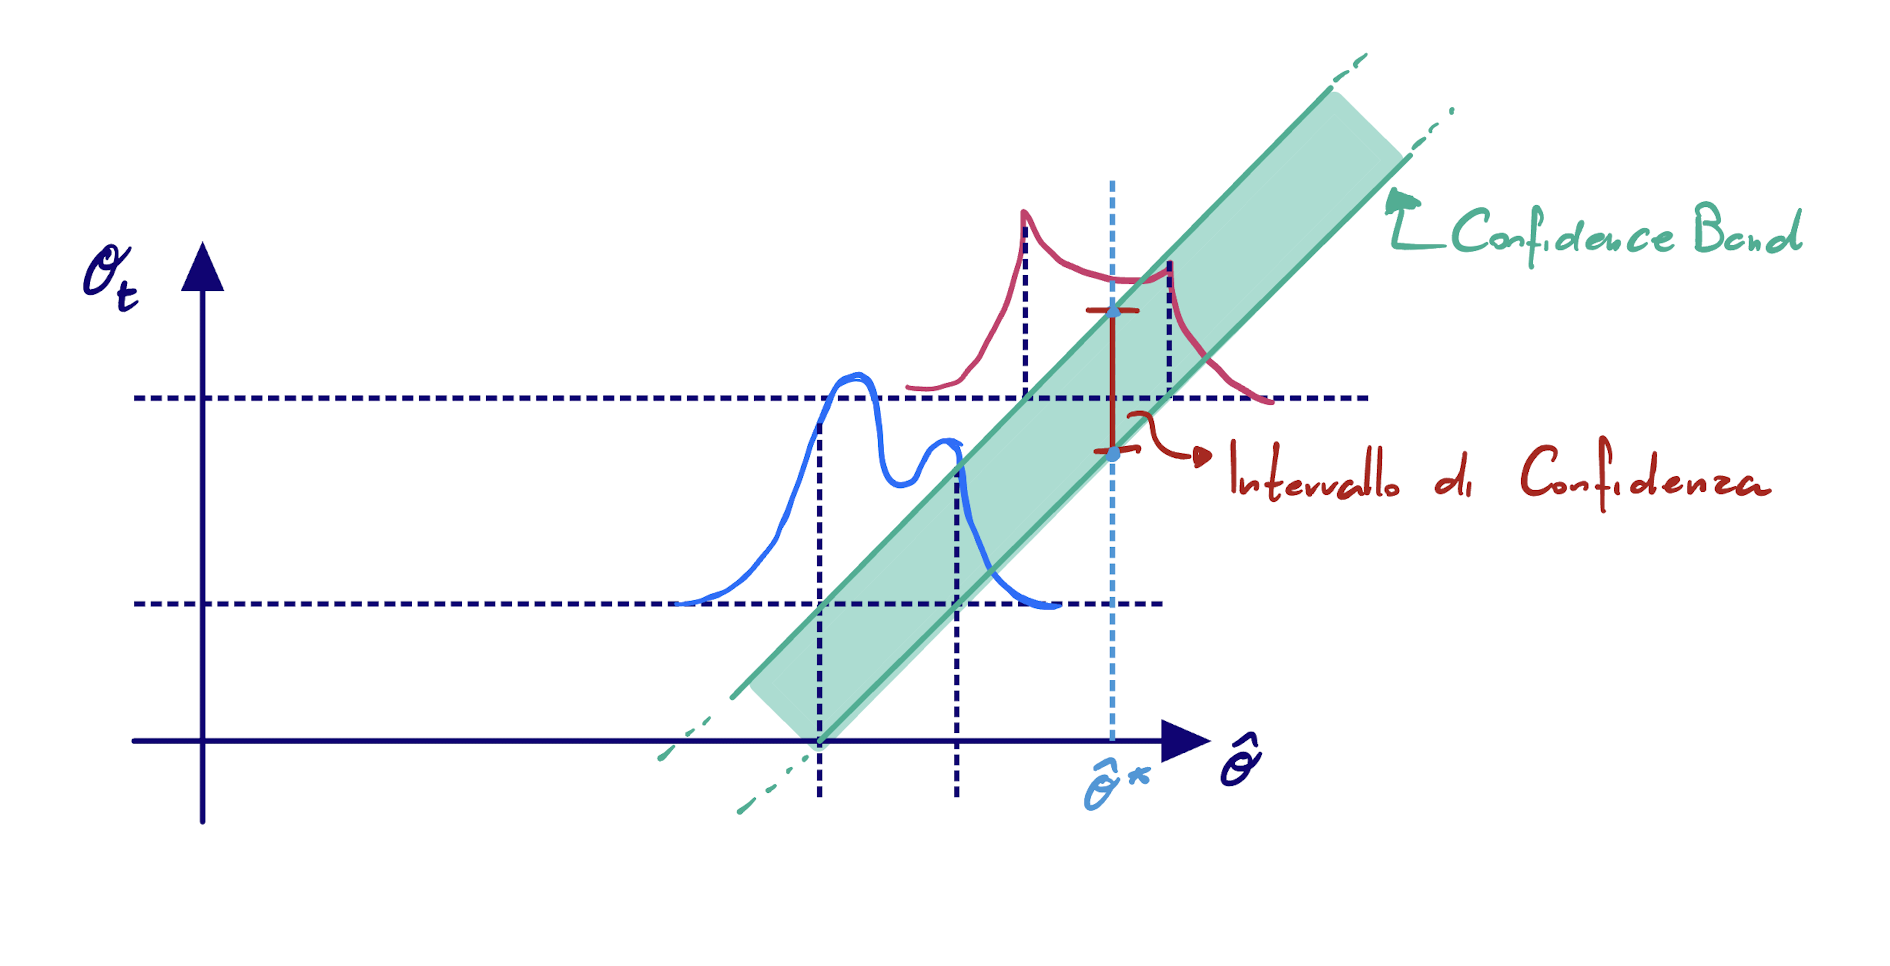
\includegraphics[scale = 0.44]{confidenceband}	
\centering
\caption{Banda di confidenza ed intervallo di confiedenza}
\end{figure}
